%!TEX root = ../DigSig2.tex
\section{Interpolation, Decimation and Oversampling\buch{Chapter 12}}
\subsection{Interpolation and Oversampling\buchSeite{632-637}}
Oversampling is increasing the sample rate and requires some form of interpolation. New samples at a higher sampling rate are created. These are calculated using a FIR filter. The spectrum of the low-rate and the high-rate signal are identical, if the frequency axis is not normalized.

\subsection{Interpolation Filter Design\buchSeite{638-657}}
\subsubsection{Direct form\buchSeite{638}}

\begin{center}
	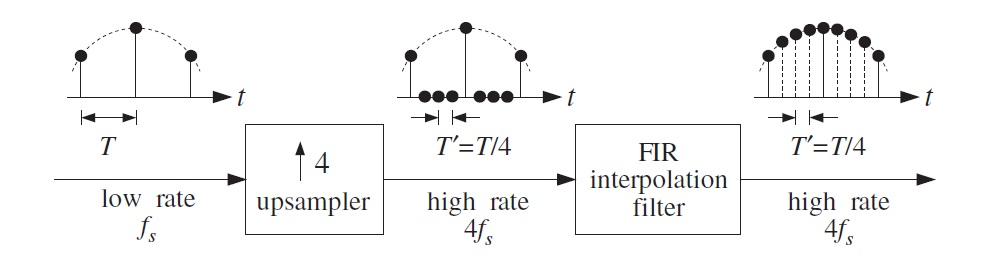
\includegraphics[width=10cm]{images/IntDecOv_IncSamplingRate.jpg}
\end{center}

There are now two discrete times, a fast one $n'$ and a slow one called $n$.
The effect on the spectrum of a signal and the advantage in DA-Conversion is
shown in the following figure (left: original spectrum, right: spectrum
at high rate).

\begin{center}
	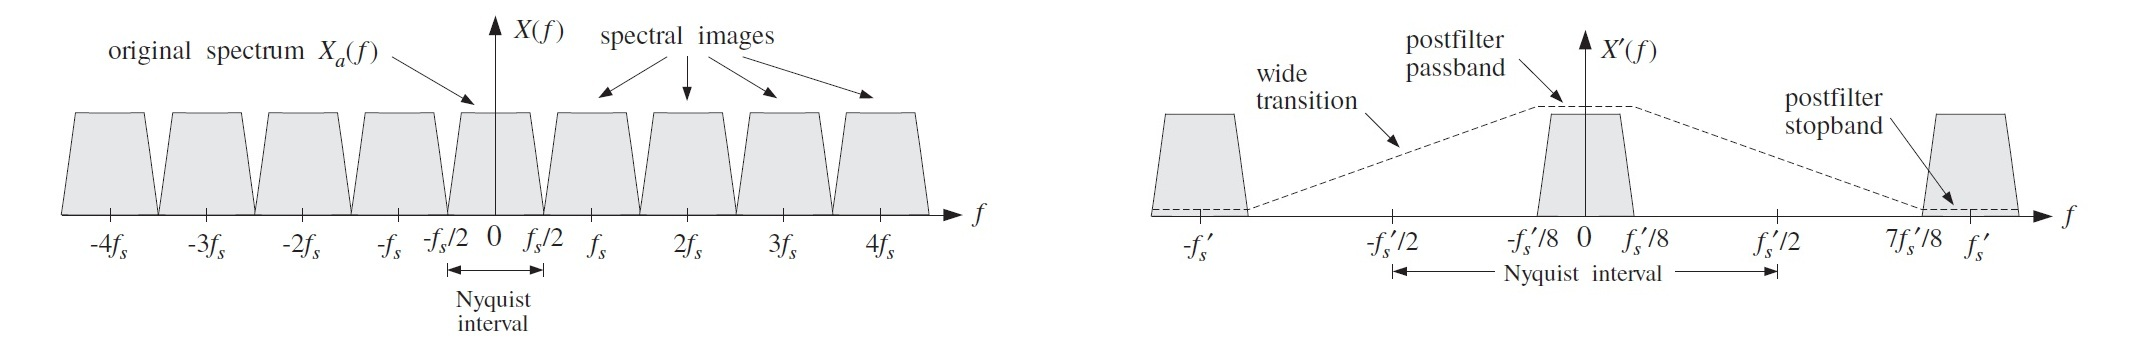
\includegraphics[width=16cm]{images/IntDecOv_Spectrum.jpg}
\end{center}

The Job of the FIR filter is to move the zeros to the appropriate values,
or to erase the spectral copies of the original spectrum in the new
Nyquist band. \\

\begin{center}
	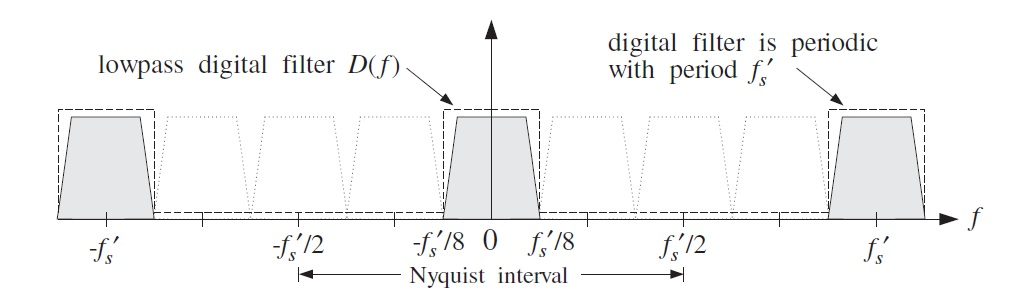
\includegraphics[width=8cm]{images/IntDecOv_Filter.jpg}
\end{center}

The ideal lowpass filter for an $L$-fold interpolation is operating at the fast
sampling rate $f'_s=L f_s$ and has its cutoff frequency at the low-sampling
rate's Nyquist frequency $f_s/2$.

\begin{equation*}
	f_c = \frac{f_s}{2}=\frac{f'_s}{2L}
	\qquad
	\omega'_c = \frac{2\pi f_c}{f'_s}=\frac{\pi}{L}
\end{equation*}

\begin{tabularx}{\linewidth}{Xl}
	FIR approximation to the ideal interpolator (non causal):
	& $d(k')=\frac{\sin(\pi k'/L)}{\pi k'/L}$, with $-LM\leq k'\leq LM$\\
	By delaying this filter by $LM$ samples, it gets causal:
	& $h(n')=d(n'-LM)=\frac{\sin(\pi (n'-LM)/L)}{\pi (n'-LM)/L}$ \\
	Using a Hamming window: & $h(n')=w(n')d(n'-LM)$ \\
	Hamming window & $w(n') = 0.54-0.46\cos(\frac{2\pi n'}{N-1})$ \\
\end{tabularx} \\

The output of the non causal FIR interpolator filter is obtained as the
convolution of the upsampled signal with the filter

\begin{equation*}
	y_{up}(n') = \sum\limits_{k'=-LM}^{LM}d(k')x_{up}(n'-k')
\end{equation*}


\subsubsection{Polyphase Form\buchSeite{640}}

\begin{multicols}{2}
	The direct form is
	\begin{center}
		\adjustbox{max width=0.7\linewidth}{\input{tikz/interpolation_direct}}
	\end{center}
\vfill\columnbreak
	A more efficient way is using the polyphase form
	\begin{center}
		\adjustbox{max width=\linewidth}{\input{tikz/interpolation_polyphase}}
	\end{center}
\end{multicols}

Note that the direct form does all multiplications at the high rate, while
the polyphase form allows doing the multiplications at the low rate, which
makes the system more efficient. \\

Suppose the low-rate time instants are $n$, then the fast-rate time instants
can be described as $n' = NL+i$ for $i=0,1,\ldots,L-1$. The output is therefore

\begin{equation*}
	y_{up}(nL+i) = \sum\limits_{k=-M}^{M-1}\sum\limits_{j=0}^{L-1} d(kL+j) x_{up}(nL+i-kL-j)
\end{equation*}

which allows us to split the output $y_{up}$ into $y_i(n)=y_{up}(nL+i)$.
We can also define the \emph{$i$th polyphase subfilter} as

\begin{equation*}
	d_i(k) = d(kL+i) \:,\qquad -M \leq k \leq M-1 \:,\quad i=0,1,\ldots,L
\end{equation*}

The $i$th outputs can now be calculated in terms of the slow-rate samples

\begin{equation*}
	y_i(n) = \sum\limits_{k=-M}^{M-1}d_i(k) x(n-k) \:,\qquad i=0,1,\ldots,L-1
\end{equation*}

The output $y_{up}$ is now only calculated in terms of the slow sampling rate,
which decreases the computational rate in terms of multiplications per second by
a factor of $L$, from $R = NLf_s$ (direct from) to $R = Nf_s$ (polyphase form).


\subsubsection{Frequency domain characteristics\buchSeite{645}}
To discuss the interpolation in the frequency domain, we introduce the different
unit delays $z$ (low sampling rate = long delay) and $\zeta$
(high sampling rate = short delay)

\begin{equation*}
	z = \zeta^L \qquad \Leftrightarrow \qquad \zeta = z^{1/L}
\end{equation*}

The high-rate output can now be written in the $z$-Domain as

\begin{equation*}
	Y_{up}(\zeta) = \sum\limits_{i=0}^{L-1} \zeta^{-i} Y_i(\zeta^L)
	= \sum\limits_{i=0}^{L-1} z^{-i/L} Y_i(z)
\end{equation*}

which is what we already know from the time domain. The filter $D(\zeta)$
similarly is

\begin{equation*}
	D(\zeta) = \sum\limits_{i=0}^{L-1} \zeta^{-i} D_i(\zeta^L)
	= \sum\limits_{i=0}^{L-1} z^{-i/L} D_i(z)
\end{equation*}

\paragraph{Low-Rate Representation}

The original low-rate signal is represented in the $z$-domain by

\[
Y(z)=H(z)X(z),
\]

where the sampling frequency is

\[
f_s.
\]

After interpolation by the factor $L$, the sampling frequency becomes

\[
f_s'=Lf_s,
\]

and the corresponding transform variable changes from

\[
z
\longrightarrow
\zeta.
\]

The high-rate output is therefore represented by

\[
Y_{up}(\zeta).
\]

\paragraph{Overall High-Rate Transfer Function}

Replacing

\[
z=\zeta^L
\]

gives the high-rate interpolation filter

\[
\boxed{
H(\zeta)
=
\sum_{i=0}^{L-1}
\zeta^{-i}H_i(\zeta^L).
}
\]

For \(L=4\),

\[
H(\zeta)
=
H_0(\zeta^4)
+\zeta^{-1}H_1(\zeta^4)
+\zeta^{-2}H_2(\zeta^4)
+\zeta^{-3}H_3(\zeta^4).
\]

The 0th polyphase subfilter $d_0(k)$ should of course return the same value as
the input $x(n)$, so the impulse response must be a dirac:
$d_0(k) = d(kL) = \delta(k)$. \\

The ideal filter which removes all spectral copies would generally have
the following characteristics
\begin{equation*}
	D(f) = \begin{cases}
		L\:,	& \text{if} \quad |f|\leq\frac{f_s}{2} \\
		0\:,	& \text{if} \quad \frac{f_s}{2}\leq |f|\leq\frac{f'_s}{2}
	\end{cases}
\end{equation*}

The ideal reconstructor $d(k)$, running at the higher rate $f_s'$ would
therefore be
\begin{equation*}
	d(k') = \frac{\sin(\pi k' / L)}{\pi k' / L}
\end{equation*}

This reconstructor is usually implemented using a Kaiser window design.

\[
\boxed{
\begin{array}{ccc}
\textbf{Low rate} && \textbf{High rate}\\[1mm]
f_s && f_s'=Lf_s\\
z && \zeta\\
Y(z) && Y_{up}(\zeta)
\end{array}
}
\]

%%%%%%%%%%%%%%%%%%%%%%%%%%%%%%%%%%%%%%%%%%%%%%%%%%%%%%%%%%%%
\subsubsection{Kaiser Design for Interpolation Filters}

For an $L$-fold interpolator the Kaiser design equations are slightly modified,
because the filter operates at the high sampling rate

\[
f_s'=Lf_s.
\]

The transition width is

\[
\Delta f=f_{stop}-f_{pass},
\]

or in normalized form

\[
\Delta F=\frac{\Delta f}{f_s}.
\]

The Kaiser parameters are

\[
D=\frac{A-7.95}{14.36},
\qquad
\alpha=0.1102(A-8.7).
\]

The required filter length is

\[
\boxed{
N-1\ge
\frac{DL}{\Delta F}
}
\]

where $N$ is rounded up to the next odd integer of the form

\[
N=2LM+1.
\]

Hence

\[
\boxed{
M=\frac{N-1}{2L}.
}
\]

The computational rate becomes

\[
\boxed{
R_{\text{direct}}
=
NLf_s,
\qquad
R_{\text{polyphase}}
=
Nf_s.
}
\]

\subsection{Linear and Hold Interpolators\buchSeite{657-661}}
The reconstructor described above is the ideal interpolator. Nevertheless
there exist simpler interpolators, such as the linear and the hold interpolators.
Not surprising, these are not as good as the ideal interpolator, but especially
at high sample rates, the advantage of less calculations overweights the
downsides.

\subsubsection{Hold Interpolator}
\begin{multicols}{2}
	\begin{align*}
		d(k') &= \begin{cases}
			1\:, & \text{if} \quad 0\leq k' \leq L -1\\
			0\:, & \text{otherwise}
		\end{cases} \\
		y_{up}(nL+i) &= x(n) \\
		D(f) &= \frac{\sin(\pi f/f_s)}{\sin(\pi f/Lf_s)}e^{-j\pi(L-1)f/(Lf_s)}
	\end{align*}

	The polyphase subfilters $d_i(k)$ will then be

	\begin{equation*}
		d_i(k) = \delta(k)
	\end{equation*}

\vfill
\columnbreak
	\begin{center}
		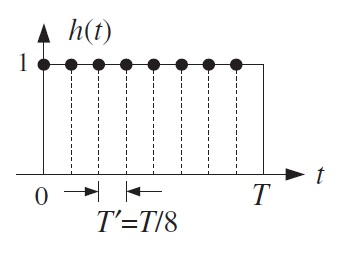
\includegraphics[width=5cm]{images/IntDecOv_Hold.jpg}
	\end{center}
\vfill
\end{multicols}

\subsubsection{Linear Interpolator}
\begin{multicols}{2}
	\begin{align*}
		d(k') &= \begin{cases}
			1-\frac{|k'|}{L}\:, & \text{if} \quad |k'|\leq L -1\\
			0\:, & \text{otherwise}
		\end{cases} \\
		y_{up}(nL+i) &= (1-\frac{i}{L})x(n)+\frac{i}{L}x(n+1) \\
		D(f) &= \frac{1}{L}\left|\frac{\sin(\pi f/f_s)}{\sin(\pi f/Lf_s)}\right|^2
	\end{align*}

	The polyphase subfilters $d_i(k)$ will then be

	\begin{equation*}
		d_i(k) = (1-\frac{i}{L}) \delta(k) + \frac{i}{L} \delta(k+1)
	\end{equation*}
\vfill
\columnbreak
	\begin{center}
		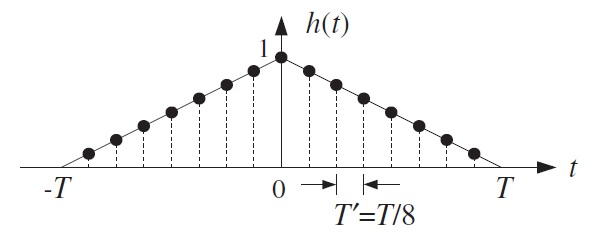
\includegraphics[width=0.8\linewidth]{images/IntDecOv_Linear.jpg}
	\end{center}
\vfill
\end{multicols}

%%%%%%%%%%%%%%%%%%%%%%%%%%%%%%%%%%%%%%%%%%%%%%%%%%%%%%%%%%%%
\paragraph{Replication Property}

The ideal interpolation filter satisfies

\[
\boxed{
\frac1L
\sum_{m=0}^{L-1}
D(f-mf_s)=1.
}
\]

Thus, the passband gain of the ideal interpolation filter must be

\[
L,
\]

which compensates for the amplitude reduction introduced by the
upsampler.

\paragraph{Interpretation}

For every frequency \(f\), exactly one replicated spectrum lies inside the
passband of the ideal interpolation filter.

Therefore,

\[
\sum_{m=0}^{L-1}D(f-mf_s)=L,
\]

and after scaling by \(1/L\),

\[
\frac1L
\sum_{m=0}^{L-1}
D(f-mf_s)=1.
\]

Hence the overall gain remains unity although the ideal interpolation filter
has a passband gain of \(L\).
\subsection{Design Examples\buchSeite{661-686}}
%TODO!!!!
\subsubsection{4-fold interpolators\buchSeite{661}}
\begin{equation*}
  L = 4
\end{equation*}
with polyphase filter length $2M=4$ or $M=2$ which leads to a filter length $N=2LM+1=17$.
The ideal impulse response is:
\begin{equation*}
  d(k')=\frac{sin(\pi k'/4)}{\pi k'/4}, \qquad -8 \leq k' \leq 8
\end{equation*}
or, numerically,
\begin{equation*}
  \mathbf{h} = \mathbf{d} = [0, -0.13, -0.21, -0.18, 0, 0.30, 0.64, 0.90, 1, 0.90, 0.64, 0.30, 0, -0.18, -0.21, -0.13, 0]
\end{equation*}
where $\mathbf{h}$ is the causal version, and $\mathbf{d}$ is the symmetric one with time origin at the middle of the vector.
The resulting polyphase subfilters
\begin{equation*}
  d_i(k) = d(4k + i), \qquad -2 \leq k \leq 1
\end{equation*}
can now be calculated (high-rate filter subsampled by a factor of 4 and an increasing offset)
\begin{align*}
  \mathbf{h}_0 &= \mathbf{d}_0 = [0, 0, 1, 0] \\
  \mathbf{h}_1 &= \mathbf{d}_1 = [-0.13, 0.30, 0.90, -0.18] \\
  \mathbf{h}_2 &= \mathbf{d}_2 = [-0.21, 0.64, 0.64, -0.21] \\
  \mathbf{h}_3 &= \mathbf{d}_3 = [-0.18, 0.90, 0.30, -0.13]
\end{align*}
\begin{center}
  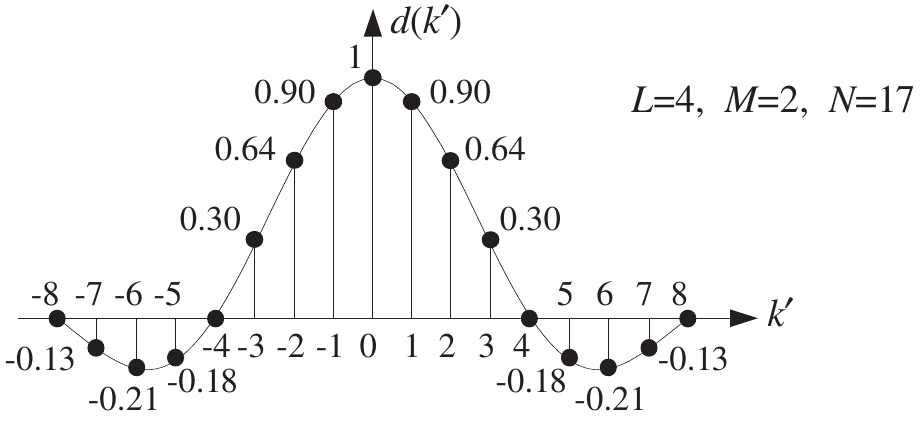
\includegraphics[width=6cm]{images/IntDecOv_DesignExample.png}
\end{center}
The interpolated samples $y_{\text{up}}(4n+i)$ between $x(n)=x_{\text{up}}(4n)$ and $x(n+1)=x_{\text{up}}(4[n+1])$ are now:
\begin{equation*}
  \begin{bmatrix}
    y_{\text{up}}(4n) \\
    y_{\text{up}}(4n+1) \\
    y_{\text{up}}(4n+2) \\
    y_{\text{up}}(4n+3)
  \end{bmatrix}
  =
  \begin{bmatrix}
        0 &    0 &    1 &     0 \\
    -0.13 & 0.30 & 0.90 & -0.18 \\
    -0.21 & 0.64 & 0.64 & -0.21 \\
    -0.18 & 0.90 & 0.30 & -0.13 \\
  \end{bmatrix}
  \begin{bmatrix}
    x_{\text{up}}(4n+8) \\
    x_{\text{up}}(4n+4) \\
    x_{\text{up}}(4n) \\
    x_{\text{up}}(4n-4)
  \end{bmatrix}
\end{equation*}
\begin{center}
  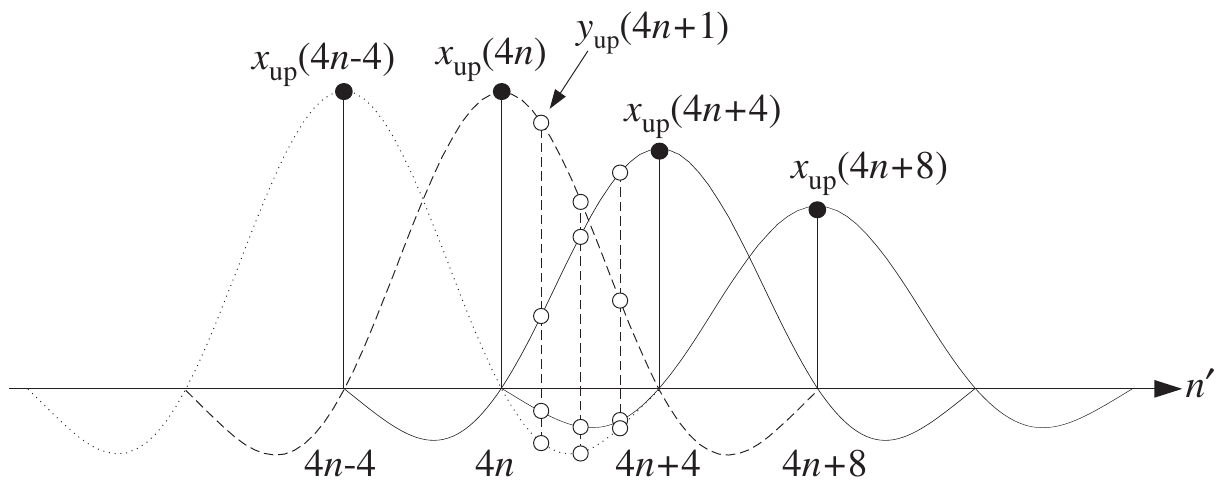
\includegraphics[width=8cm]{images/IntDecOv_DesignExampleSuperposition.png}
\end{center}

The 17 sample long FIR filter is very short ($M=2$).
This and the rectangular window have the effect that the interpolated signal is of low quality.
Rectangular windows should not be used, Hamming is much better and results in a reasonable interpolation even with $M=2$

The Hamming windowed version is obtained by multiplying the high-rate 17 sample long filter with the appropriate Hamming window resulting in
\begin{equation*}
  \begin{bmatrix}
    y_{\text{up}}(4n) \\
    y_{\text{up}}(4n+1) \\
    y_{\text{up}}(4n+2) \\
    y_{\text{up}}(4n+3)
  \end{bmatrix}
  =
  \begin{bmatrix}
        0 &    0 &    1 &     0 \\
    -0.02 & 0.22 & 0.87 & -0.07 \\
    -0.05 & 0.55 & 0.55 & -0.05 \\
    -0.07 & 0.87 & 0.22 & -0.02 \\
  \end{bmatrix}
  \begin{bmatrix}
    x_{\text{up}}(4n+8) \\
    x_{\text{up}}(4n+4) \\
    x_{\text{up}}(4n) \\
    x_{\text{up}}(4n-4)
  \end{bmatrix}
\end{equation*}

\paragraph{Important Property}

For ideal interpolation

\[
d_0(k)=\delta(k)
\]

therefore

\[
y_{up}(Ln)=x(n).
\]

Only the inserted samples are interpolated.

The resulting magnitude response shows, that the rectangular filter is steeper, at the high cost of 8.9\% overshoot, which the Hamming window version doesn't have.\\

For a block diagram realization of the polyphase form, recall these two relationships:
\begin{align*}
  Y_{\text{up}}(\xi) &= \sum_{i=0}^{L-1}\xi^{-1}Y_i(\xi^L) = \sum_{i=0}^{L-1}z^{-i/L}Y_i(z) \\
  D(\xi) &= \sum_{i=0}^{L-1}\xi^{-1}D_i(\xi^L) = \sum_{i=0}^{L-1}z^{-i/L}D_i(z)
\end{align*}
Therefore the transfer function of the high-rate interpolator filter can be written as the sum of the polyphase subfilters appropriately delayed:
\begin{align*}
  H(\xi) &= H_0(\xi^4) + \xi^{-1}H_1(\xi^4) + \xi^{-2}H_2(\xi^4) + \xi^{-3}H_3(\xi^4) \\
  &= H_0(z) + z^{-1/4}H_1(z) + z^{-2/4}H_2(z) + z^{-3/4}H_3(z)
\end{align*}
The resulting block diagram clearly shows how the four polyphase filters create the four output values.
Three of these values are interpolated while value $y_{\text{up}}(n') = y_{\text{up}}(4n) = y_0(n)$ is identical to the upsampled input value $x_{\text{up}}(n') = x_{\text{up}}(4n) = x(n)$, since $h_0=[0,0,1,0]$.
Clearly, the four output samples can be calculated in parallel, allowing for a very fast implementation.
\begin{center}
  \begin{tikzpicture}
    \node [inner sep=0pt,above right]
    {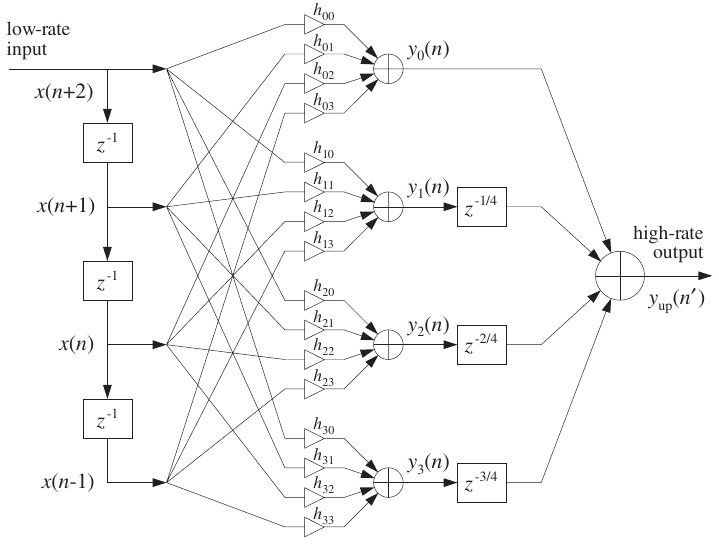
\includegraphics[width=10cm]{images/IntDecOv_DesignExamplePolyphase.png}};
    \draw[red,->] (9,7) node [right] {Missing upsampler by a factor of 4} -- (6,6.65) node {};
    \draw[red,->] (9,7) node {} -- (6,4.7) {};
    \draw[red,->] (9,7) node {} -- (6,2.75) {};
    \draw[red,->] (9,7) node {} -- (6,0.85) {};
  \end{tikzpicture}
\end{center}

\subsection{Decimation and Oversampling\buchSeite{686-691}}
Decimation is the inverse of oversampling, thus the sampling rate is reduced
from a high rate $f_s'$ to a low rate $f_s = f_s' / L$.

\begin{center}
	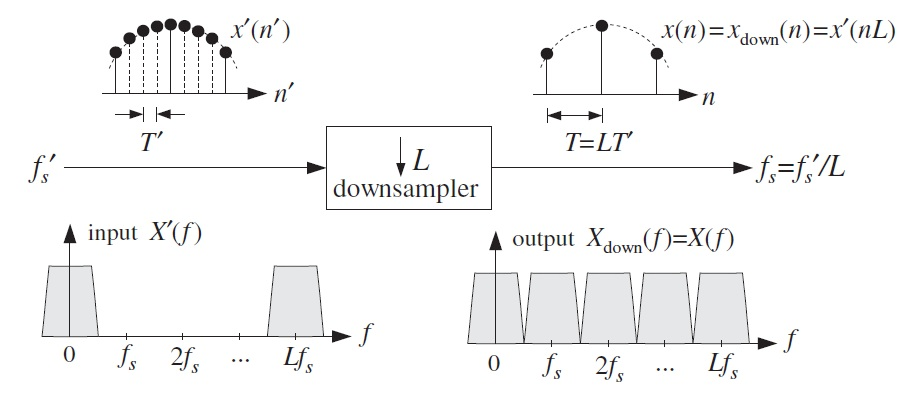
\includegraphics[width=10cm]{images/IntDecOv_Downsampler.jpg}
\end{center}

Downsampling is simply the process of discarding $L-1$ samples:

\begin{equation*}
	x_{down}(n) = \left.x'(n')\right|_{n'=nL} = x'(nL)
\end{equation*}
%%%%%%%%%%%%%%%%%%%%%%%%%%%%%%%%%%%%%%%%%%%%%%%%%%%%%%%%%%%%
\paragraph{Frequency-Domain Relation}

Downsampling causes a periodic replication of the high-rate spectrum:

\[
\boxed{
X(f)
=
\frac1L
\sum_{m=0}^{L-1}
X'(f-mf_s).
}
\]

Using normalized digital frequency

\[
\omega=\frac{2\pi f}{f_s},
\]

this becomes

\[
\boxed{
X(\omega)
=
\frac1L
\sum_{m=0}^{L-1}
X'
\left(
\omega'
-
\frac{2\pi m}{L}
\right).
}
\]
\paragraph{Proof Idea (Problem 12.12)}

Starting from the two Poisson summation formulas

\[
X(f)=\frac1T\sum_{k=-\infty}^{\infty}X_a(f-kf_s),
\qquad
X'(f)=\frac1{T'}\sum_{k'=-\infty}^{\infty}X_a(f-k'f_s'),
\]

use the substitution

\[
k=Lk'+m,\qquad m=0,\ldots,L-1,
\]

together with

\[
f_s'=Lf_s,
\qquad
T=LT',
\]

to obtain

\[
X(f)=
\frac1L
\sum_{m=0}^{L-1}
X'(f-mf_s).
\]

The factor \(1/L\) compensates for the sum of the \(L\) replicated spectra.

Caution: if the high rate spectrum occupies more than the low rate Nyquist rate
there \emph{will} be aliasing. \\

The ideal \emph{decimator} therefore contains a decimation filter, which
operates at the high frequencies and cuts out the low rate Nyquist band.

\begin{center}
	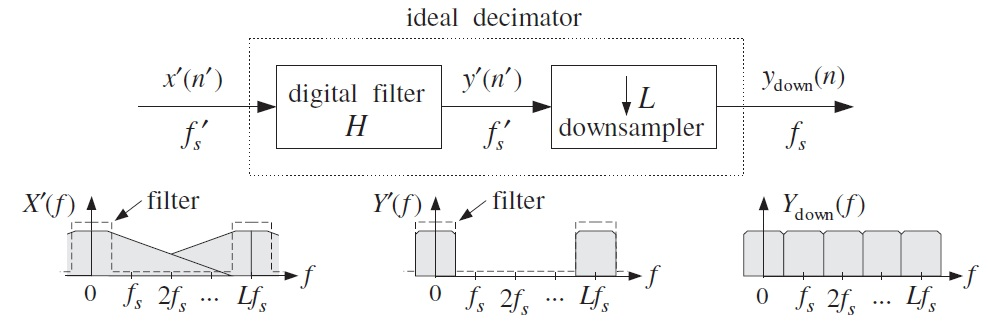
\includegraphics[width=12cm]{images/IntDecOv_Decimator.jpg}
\end{center}

The decimation filter is similar to the interpolation filter, except that
its DC gain is unity instead of $L$. A length-$N$ FIR decimation filter
can therefore be obtained by

\begin{equation*}
	h(n') = w(n') d(n'-LM) \:,\qquad \text{where} \quad
	d(k') = \frac{\sin(\pi k'/L)}{\pi k'}
\end{equation*}

Since only every $L$th output sample is needed, the filter output does
not need to be calculated for every fast rate sample (like on the left image),
reducing the computational cost by a factor $L$ to
$R = \frac{1}{L} N f_s' = N f_s$ (left image). \\

\begin{multicols}{2}
	\begin{center}
		\adjustbox{max width=0.9\linewidth}{\input{tikz/decimation}} \\
	\end{center}
\vfill\columnbreak
	\begin{center}
		\adjustbox{max width=0.7\linewidth}{\input{tikz/decimation_polyphase}} \\
	\end{center}
\end{multicols}

Multistage designs are very popular for decimation filters. The early filters will
then be fast but simple, while later filters are slow but very precise. For fast
signals, often a simple FIR averaging filter is used. The last, slowest filter
can then be designed to fix the overall frequency response.
\paragraph{Butterworth Attenuation}

For an analog Butterworth filter

\[
A(F)
=
10\log_{10}
\!\left(
1+
\left(\frac{F}{F_0}\right)^{2N}
\right),
\]

where

\[
F=\frac{f}{f_s},
\qquad
F_0=\frac{f_0}{f_s}.
\]

For oversampling prefilters

\[
F_{pass}=0.5,
\qquad
F_{stop}=L-0.5.
\]

%%%%%%%%%%%%%%%%%%%%%%%%%%%%%%%%%%%%%%%%%%%%%%%%%%%%%%%%%%%%
\paragraph{Oversampling Ratio}

For a third-order Butterworth analog antialiasing prefilter,

\[
\boxed{
L
\approx
0.94\cdot10^{A_{stop}/60}+0.5
}
\]

gives the minimum oversampling ratio required to achieve a stopband
attenuation of \(A_{stop}\).

%%%%%%%%%%%%%%%%%%%%%%%%%%%%%%%%%%%%%%%%%%%%%%%%%%%%%%%%%%%%
\paragraph{Butterworth Prefilter Order}

The required order of the analog Butterworth antialiasing filter is

\[
\boxed{
N
=
\frac{
\ln
\left(
\dfrac{10^{A_{stop}/10}-1}
      {10^{A_{pass}/10}-1}
\right)
}
{
2\ln(2L-1)
}
}
\]

The filter order decreases as the oversampling factor \(L\) increases.

\subsection{Noise Shaping Quantizer\buchSeite{698-705}}

%%%%%%%%%%%%%%%%%%%%%%%%%%%%%%%%%%%%%%%%%%%%%%%%%%%%%%%%%%%%
\paragraph{First-Order Delta-Sigma A/D Converters}

For first-order delta-sigma A/D converters, only one output bit is used
($B'=1$). By oversampling the input signal, the quantization noise is
shifted towards higher frequencies, where it is removed by the digital
decimation filter.

\begin{center}
	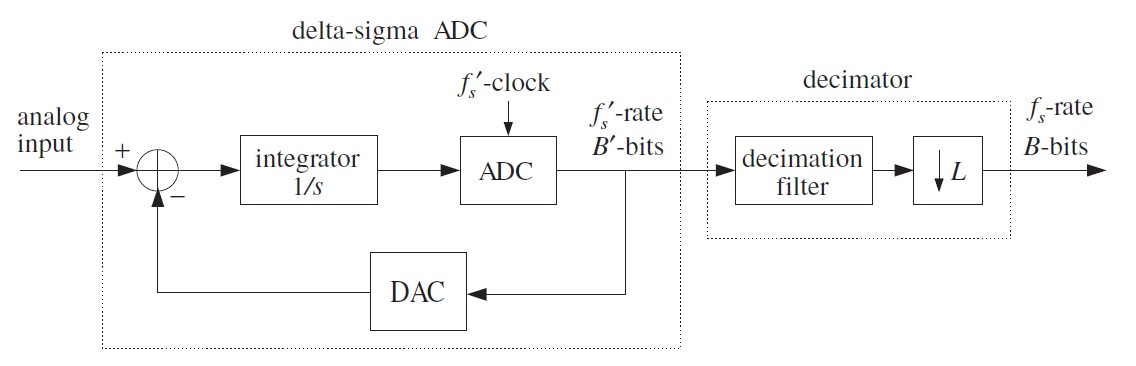
\includegraphics[width=11cm]{images/IntDecOv_SigmaDelta.jpg}
\end{center}

To obtain a discrete-time model, the quantizer is replaced by an
equivalent additive quantization noise source.

\begin{center}
	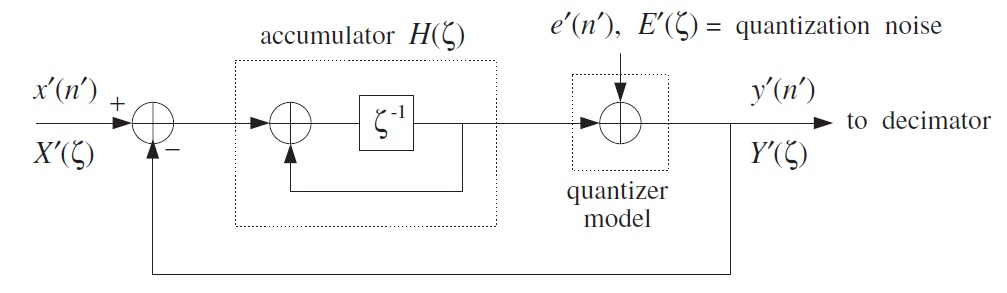
\includegraphics[width=10cm]{images/IntDecOv_SigmaDeltaModel.jpg}
\end{center}

%%%%%%%%%%%%%%%%%%%%%%%%%%%%%%%%%%%%%%%%%%%%%%%%%%%%%%%%%%%%
\paragraph{General Signal and Noise Transfer Functions}

For a loop filter $H(\zeta)$, the input and noise transfer functions are

\[
\boxed{
H_X(\zeta)=\frac{H(\zeta)}{1+H(\zeta)}
}
\]

\[
\boxed{
H_{NS}(\zeta)=\frac{1}{1+H(\zeta)}
}
\]

These relations are valid for arbitrary noise-shaping loops.

%%%%%%%%%%%%%%%%%%%%%%%%%%%%%%%%%%%%%%%%%%%%%%%%%%%%%%%%%%%%
\paragraph{First-Order Noise Shaping}

For the first-order accumulator

\[
H(\zeta)=\frac{\zeta^{-1}}{1-\zeta^{-1}}
\]

the transfer functions become

\[
\boxed{
H_X(\zeta)=\zeta^{-1}
}
\]

\[
\boxed{
H_{NS}(\zeta)=1-\zeta^{-1}.
}
\]

%%%%%%%%%%%%%%%%%%%%%%%%%%%%%%%%%%%%%%%%%%%%%%%%%%%%%%%%%%%%
\paragraph{Higher-Order Noise Shaping}

For a noise shaper of order $p$

\[
\boxed{
H_{NS}(\zeta)=\left(1-\zeta^{-1}\right)^p.
}
\]

For the second-order case,

\[
H_{NS}(\zeta)=\left(1-\zeta^{-1}\right)^2.
\]

%%%%%%%%%%%%%%%%%%%%%%%%%%%%%%%%%%%%%%%%%%%%%%%%%%%%%%%%%%%%
\paragraph{Quantization Noise Power}

The mean-square quantization noise is

\[
\sigma_e^2
=
\sigma_{e'}^2
\frac{1}{f_s'}
\int_{-f_s/2}^{f_s/2}
|H_{NS}(f)|^2\,df,
\]

where

\[
f_s'=Lf_s.
\]

The magnitude response of the noise shaping filter is

\[
|H_{NS}(f)|^2
=
\left(
\frac{\pi^{2p}}{2p+1}
\right).
\]

This leads to the well-known resolution improvement

\[
\boxed{
\Delta B
=
(p+0.5)\log_2L
-
\frac12
\log_2
\left(
\frac{\pi^{2p}}{2p+1}
\right).
}
\]

%%%%%%%%%%%%%%%%%%%%%%%%%%%%%%%%%%%%%%%%%%%%%%%%%%%%%%%%%%%%
\paragraph{Oversampled Noise-Shaping Requantizers for D/A Conversion}

The same principle can also be applied to D/A conversion.

\begin{center}
	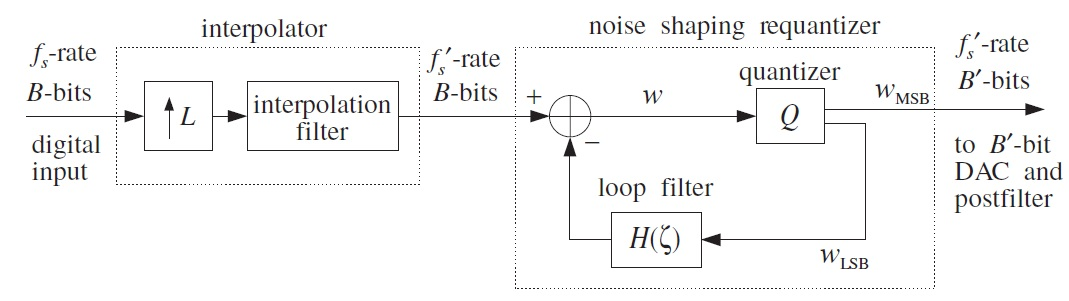
\includegraphics[width=12cm]{images/IntDecOv_Requantizer.jpg}
\end{center}

Typical loop filters are

\[
\begin{aligned}
\text{First-order:}\qquad
&H(\zeta)=\zeta^{-1},
&
H_{NS}(\zeta)=1-\zeta^{-1},
\\[1ex]
\text{Second-order:}\qquad
&H(\zeta)=2\zeta^{-1}-\zeta^{-2},
&
H_{NS}(\zeta)=\left(1-\zeta^{-1}\right)^2.
\end{aligned}
\]

The achievable resolution improvement is again

\[
\boxed{
\Delta B
=
(p+0.5)\log_2L
-
\frac12
\log_2
\left(
\frac{\pi^{2p}}{2p+1}
\right).
}
\]